Um die Umsetzbarkeit diese Projektes zu überprüfen, wurde ein Prototyp angefertigt.\\
\\
Aus einem alten Schlauchboot wurde der Boden entfernt. Danach wurde aus einer Holzplatte mittig ein Loch ausgeschnitten und der Motor mit Propeller wurde darüber montiert -- siehe \autoref{fig:ErsterPrototyp}.
\begin{figure}[h!]
  \centering
  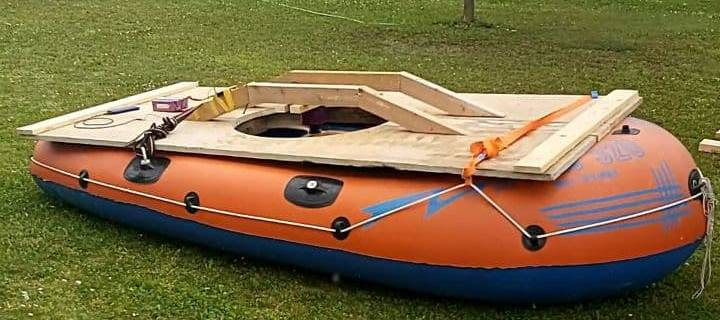
\includegraphics[width=.95\textwidth]{./Aufbau1.jpg}
  \caption{Aufbau erster Prototyp}
  \label{fig:ErsterPrototyp}
\end{figure}

Der Motorregler wurde direkt an zwei in Serie geschaltete 6S-LiPo Akkus angeschlossen und mit einer Fernbedienung gesteuert.
\section*{Erkenntnisse}
Der Test hat gezeigt, dass unser Motor mit dem verwendeten Propeller genug Kraft hat, um einen erwachsenen Menschen zu tragen. Dies bedeutet, dass der Bau eines Luftkissenboots nach unserem Plan möglich ist. Durch die großen Luftspalten zwischen der Holzplatte und dem Schlauchboot ging sehr viel Luft verloren, was die Effizienz stark verschlechterte. Deshalb schließen wir in unserer fertigen Konstruktion diese Luftspalten mittels Teichfolie. 
